%\section{\centering Experimental Setup}
\chapter{Summary and Outlook}
%\chapter*{\centering Experimental Setup}
\label{ch:Summary}

This thesis presents a search for a narrow massive resonance decaying to a pair of Higgs bosons in the four b quark final state using the LHC proton-proton collision data collected at a center-of-mass energy of 13 TeV by the CMS detector, and corresponding to an integrated luminosity of 35.9 $\mathrm{fb}^{-1}$. The $H\rightarrow bb$ decays are reconstructed as large-area jets and identified using jet substructure and b-tagging techniques. The main background is multijet production through QCD interactions and is estimated entirely from the data. The data is found to be consistent with the standard model expectations and therefore upper limits are set on the products of the resonant production cross sections of a Kaluza-Klein bulk graviton and a Randall-Sundrum radion, and their branching fraction to $\mathrm{HH}\rightarrow \mathrm{b\bar{b}b\bar{b}}$. The limits range from 126 to 1.4 fb at $95\%$ confidence level for bulk gravitons and radions in the mass range $750-3000$ GeV. For the mass scale $\Lambda_{R} = 3$ TeV, a radion of mass between 970 and 1400 GeV is excluded. The expected limits on the radion and bulk graviton for all resonant HH searches done at CMS with 2016 data can be seen in Figure~\ref{fig:HHresults} and for resonance masses $> 1100$ GeV the limits from this analysis are the most stringent. Ongoing work is currently being done by the CMS Collaboration to improve the limits by combining all of these HH search channels, although the inclusion of the $\mathrm{b\bar{b}}\gamma\gamma$ channel will only neglibly improve the sensitivity at high resonance masses due to the strength of the $\mathrm{b\bar{b}b\bar{b}}$ channel.

\begin{figure}[h!]
\centering
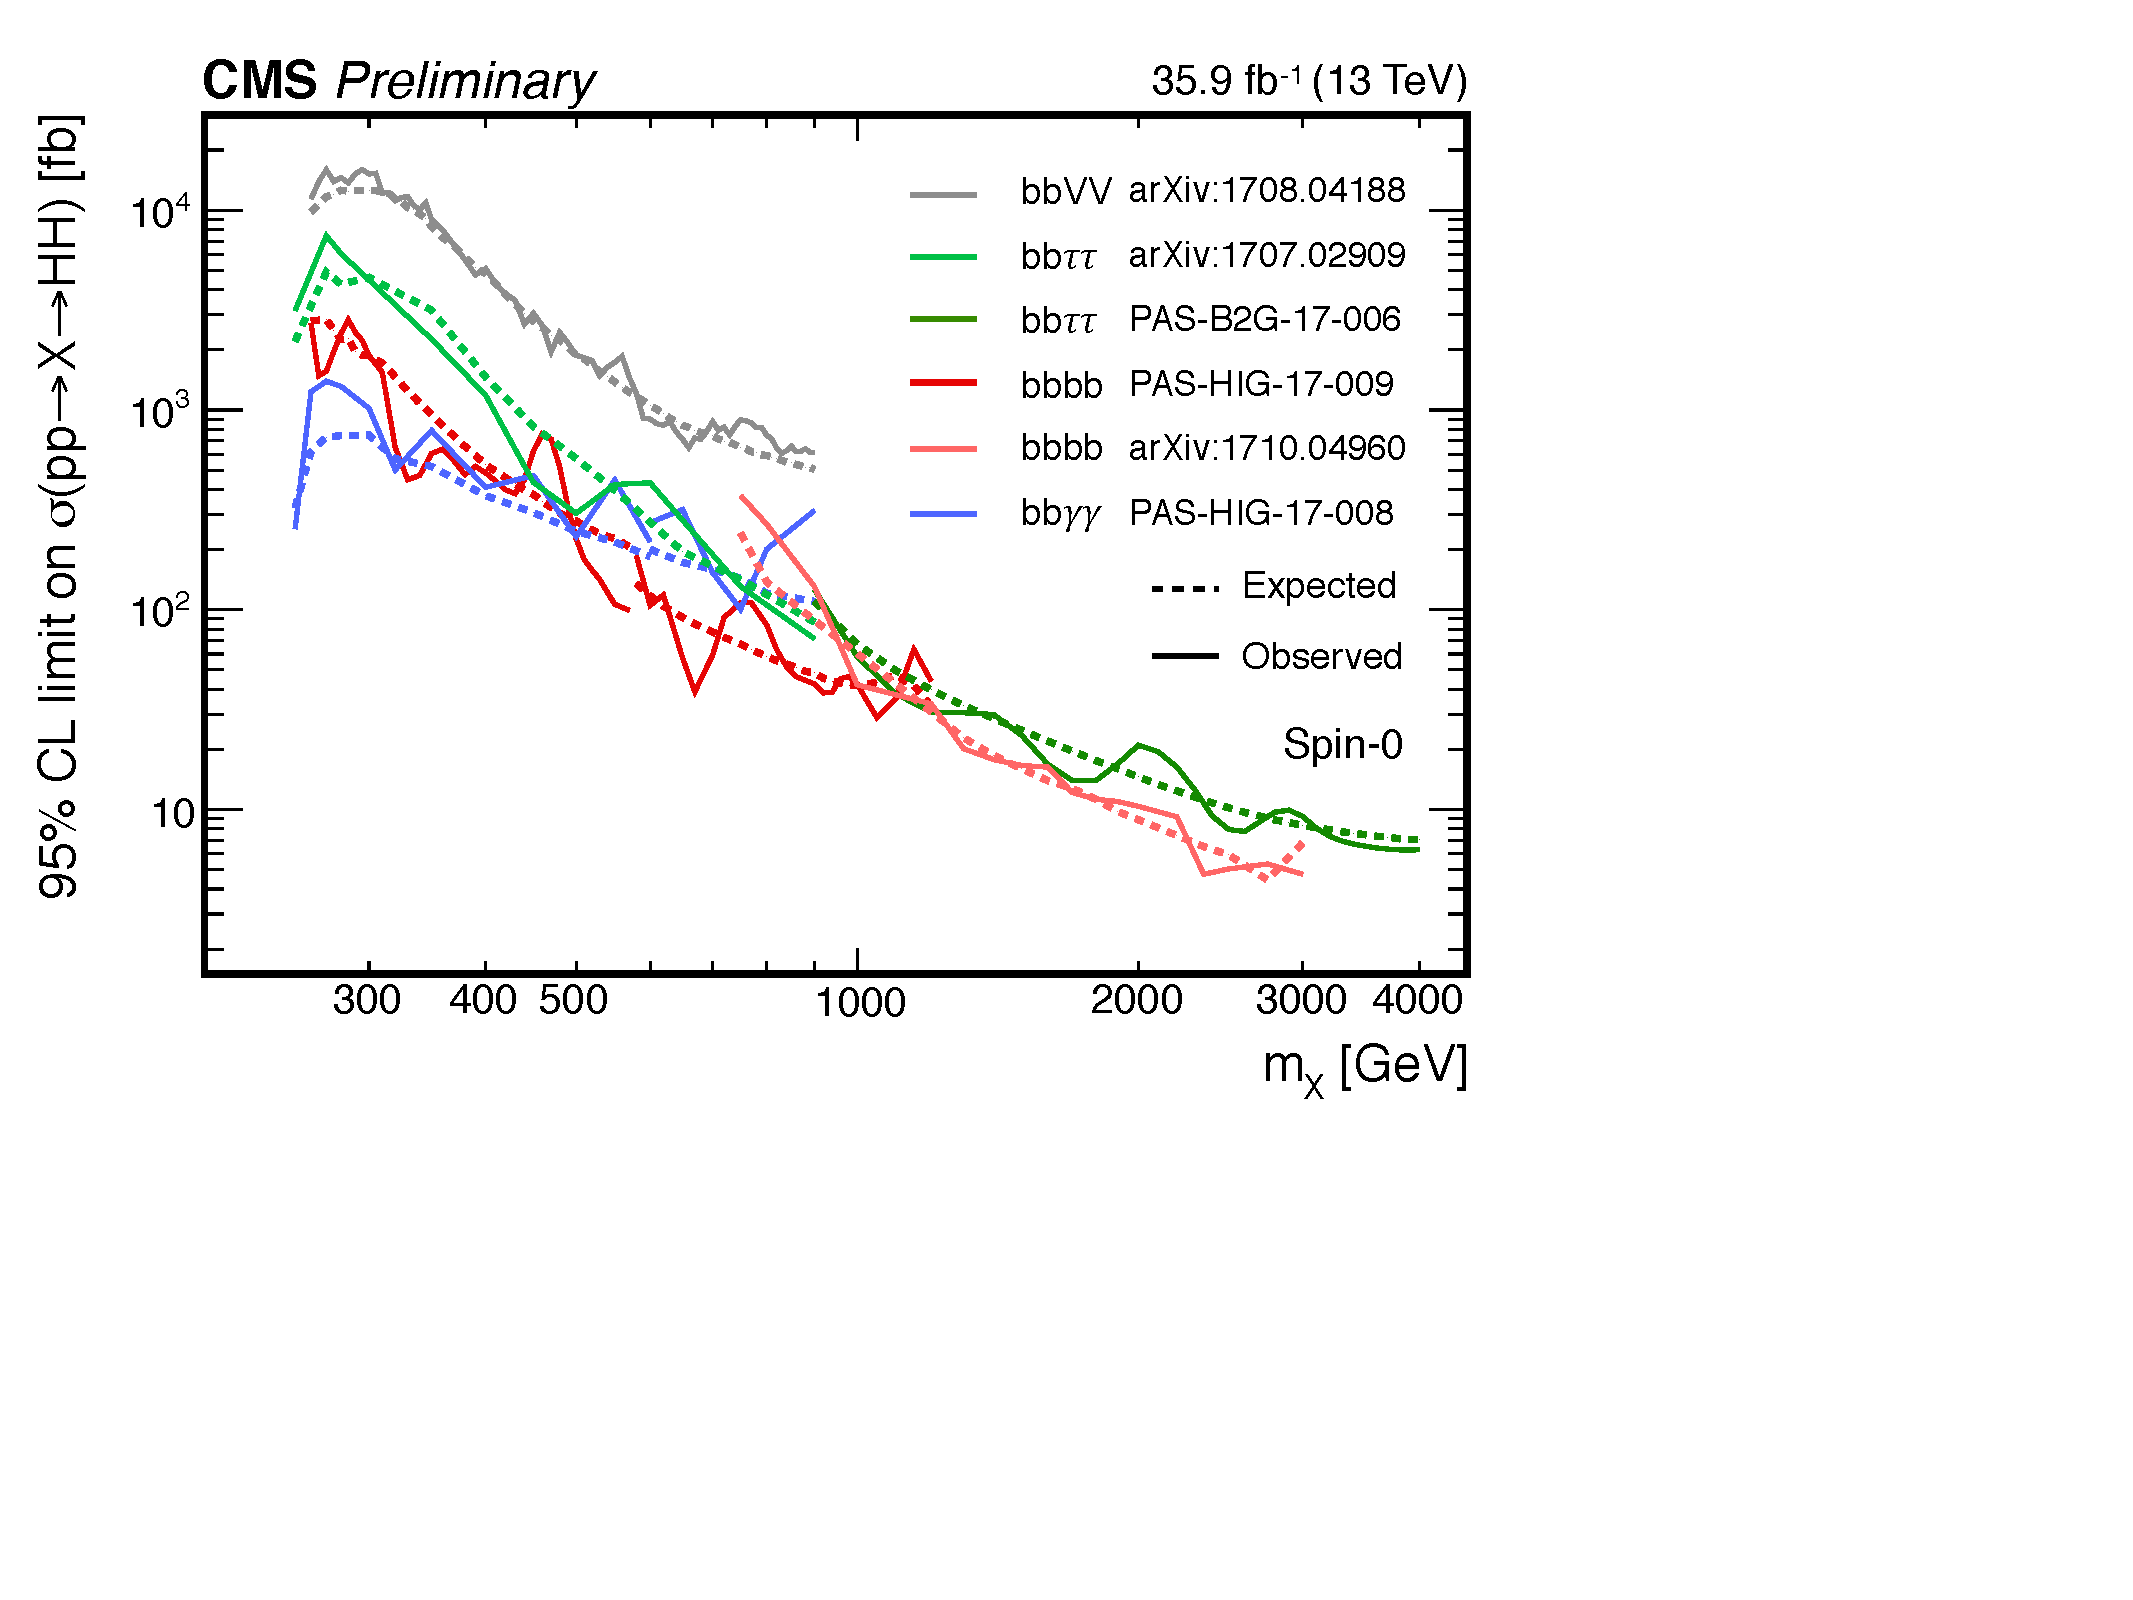
\includegraphics[width=0.45\textwidth]{Conclusion/HH_Common_plot_spin0.pdf}
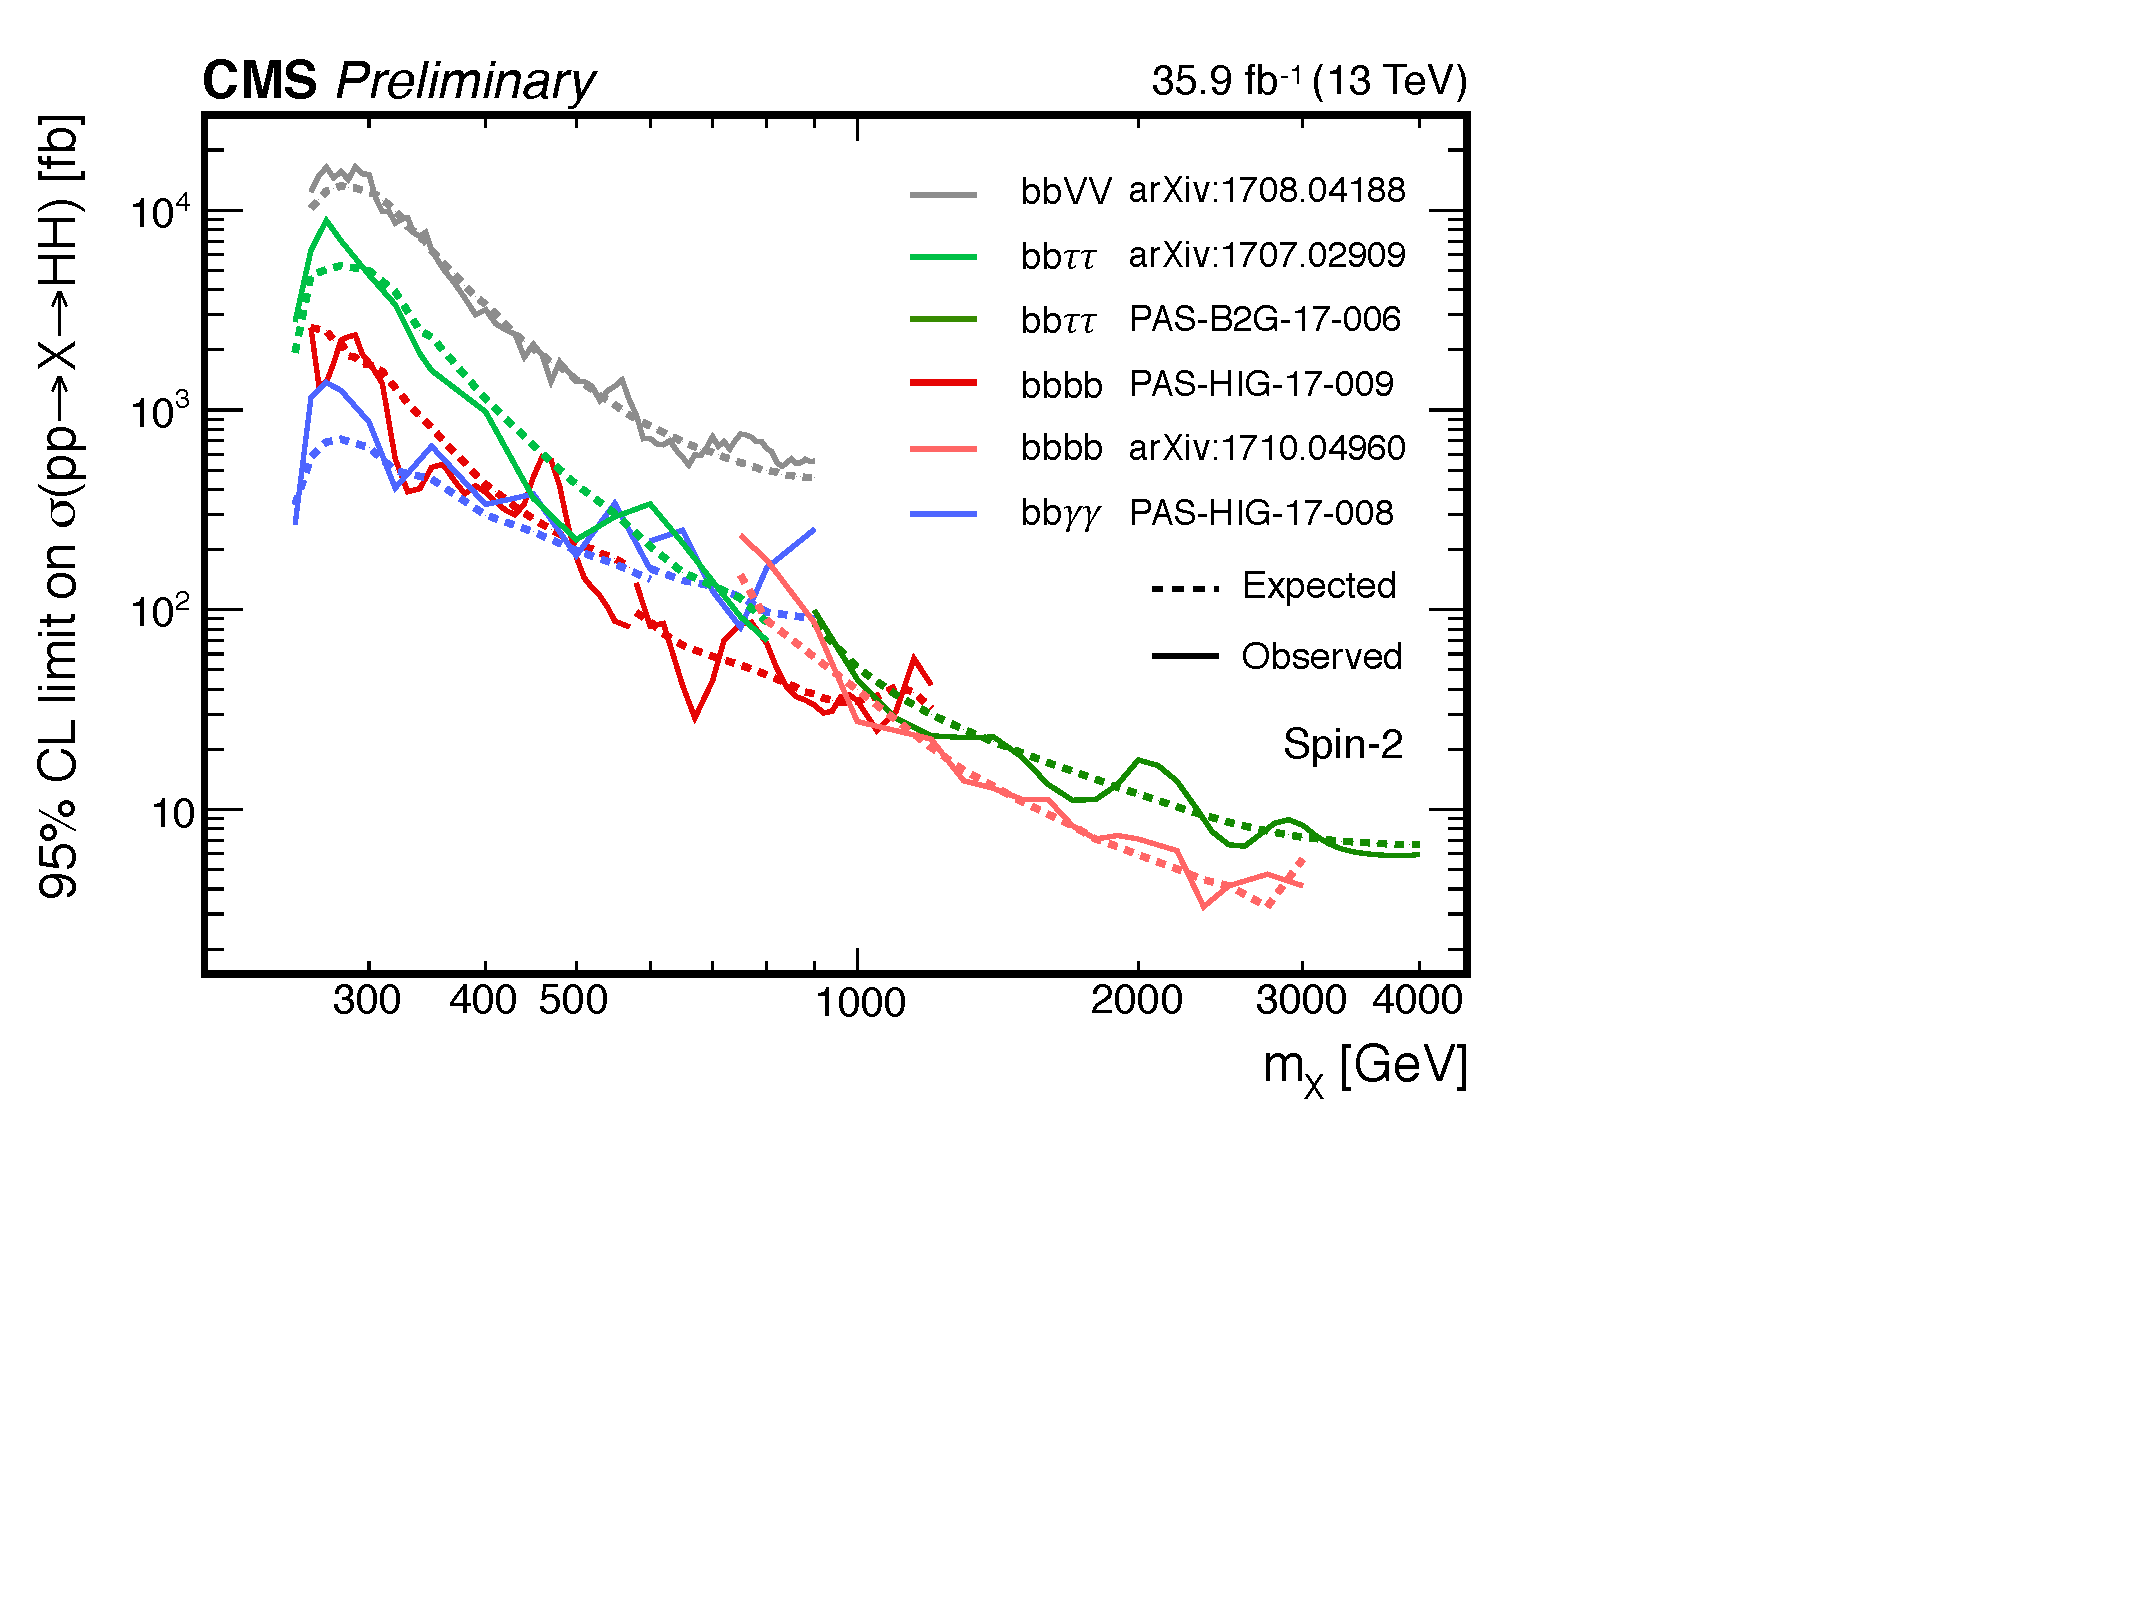
\includegraphics[width=0.45\textwidth]{Conclusion/HH_Common_plot_spin2.pdf}
\caption{The limits for the spin-0 radion (left) and the spin-2 bulk graviton (right) from all resonant HH final states searched for with the CMS detector in the full 2016 dataset.}
\label{fig:HHresults}
\end{figure}

By the end of 2018, the CMS detector will have collected ${\sim}130$ $\mathrm{fb}^{-1}$ of 13 TeV data and the sensitivity of the $\mathrm{HH}\rightarrow \mathrm{b\bar{b}b\bar{b}}$ search will be improved by utilizing this full dataset. A recent development within the CMS collaboration that could further improve the sensitivity of this search is the development of a new double-b tagger. This double-b tagger is created from a deep neural network to improve on the signal discrimination from the double-b tagger used in this analysis. Initial studies have found that at the same QCD mistag rate the new double-b tagger doubles the tagging efficiency of $\mathrm{H}\rightarrow \mathrm{b\bar{b}}$ events. The increase in sensitivity of this analysis would be greatly improved by increasing the discrimination between QCD background and $\mathrm{HH}$ signal events. 

Looking further into the future, the plan for the LHC is to shut down for over two years after the 2018 data taking period in preparation for a slight increase to the center-of-mass energy to 14 TeV and the CMS detector is expected to collect ${\sim}300$ $\mathrm{fb}^{-1}$ of data at this energy. Then another shut down will occur in preparation for the HL-LHC which will begin running in 2026 and is expected to collect ${\sim}3000$ $\mathrm{fb}^{-1}$. In order for the CMS detector to be able to handle the large amount of pileup at the HL-LHC, where it will increase to at least 140 compared to the $45-60$ that was obtained during 2016, the pixel detector will have to be completely replaced. The radiation studies presented in this thesis indicate that 65 nm CMOS technology is a viable technology for the HL-LHC pixel detector and would allow the pixel detector to function throughout the lifetime of the HL-LHC. 

With this increase in center-of-mass energy and the large amount of expected data, hopefully searches for resonant HH production will be able produce a discovery at the LHC. In the scenario that no discovery is made, resonant and non-resonant HH searches will be able to place precise constraints on SM HH production and possibly determine the Higgs self-coupling, $\lambda_{\mathrm{HHH}}$. Projections have been done that predict the CMS detector will be able to measure $\lambda_{\mathrm{HHH}}$ with a significance of $0.9\sigma$ with 3000 $\mathrm{fb}^{-1}$ of data by combining the $bb\tau\tau$ and $bb\gamma\gamma$ search channels~\cite{HLLHC}. However, including other search channels, such as $\mathrm{b\bar{b}b\bar{b}}$ where the backgrounds have been much more manageable than expected due to double-b tagging, in the combination will increase the significance and furthermore, unforeseen improvements to analysis techniques could further push this significance to a discovery. Therefore, I am optimistic that a discovery of SM HH production is feasible within the current expected lifetime of the LHC.
